\documentclass{beamer}

\usepackage[utf8]{inputenc}

\usepackage{color}
\usepackage{listings}
\usepackage{tikz}
\usepackage{hyperref}

\usetheme{Rochester}
\usecolortheme{beaver}

\lstloadlanguages{[5.2]Lua,C++}
    \lstset{%
        language={[5.2]Lua},
        basicstyle=\ttfamily,
        keywordstyle=\color{blue},
        showstringspaces=false,
        escapechar={§},
        escapeinside=||
    }

\newif\iftransitions
% \transitionstrue


\title{Howling at the Moon:}
\subtitle{Lua for C++ Programmers}
\author{Andreas Weis}
\institute{BMW AG}
\date{cppcon, September 29, 2017}
\titlegraphic{
\includegraphics[height=.25\textheight]{resources/cppcon.png}}


\begin{document}

\frame{\titlepage}

\begin{frame}[fragile]
  \frametitle{About me}

  \begin{itemize}
    \setlength\itemsep{1.5em}

    \item \href{https://stackoverflow.com/users/577603/comicsansms}{
\includegraphics[height=.05\textheight]{resources/so-icon.png}} \href{https://github.com/ComicSansMS}{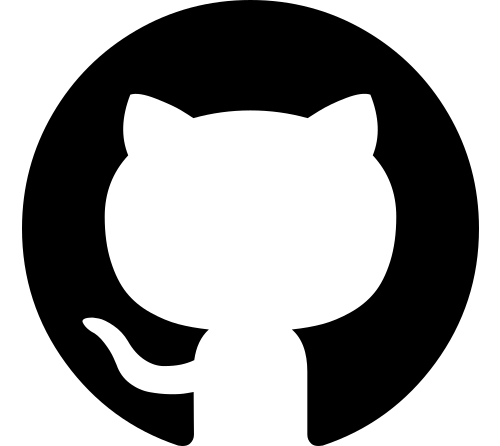
\includegraphics[height=.05\textheight]{resources/github-icon.png}} 
\includegraphics[height=.05\textheight]{resources/slack-icon.png} Known as ComicSansMS on most sites

    \item \href{https://twitter.com/DerGhulbus/}{
\includegraphics[height=.05\textheight]{resources/twitter-icon.png} @DerGhulbus on Twitter}

    \item 
\includegraphics[height=.05\textheight]{resources/meetup-icon.png} Co-organizer of the \href{https://www.meetup.com/MUCplusplus/}{Munich C++ User Group}

    \item Currently working as a Software Architect for BMW 
\includegraphics[height=.1\textheight]{resources/bmw_group.jpg}

  \end{itemize}
\end{frame}

\begin{frame}[fragile]

  \begin{center}
    \href{http://www.lua.org/}{
\includegraphics[height=.8\textheight]{resources/lua-logo.png}}
  \end{center}

\end{frame}

\begin{frame}[fragile]
  \frametitle{Lua}

  \begin{quote}Lua is a powerful, efficient, lightweight, embeddable scripting language.\end{quote}

  \pause

  \begin{itemize}
    \item Powerful
    \item Efficient
    \item Lightweight
    \item Embeddable
  \end{itemize}

  \begin{itemize}
  \item Powerful - First-class functions w/ full lexical scoping; Support for OOP paradigms; Metaprogramming; Reflection
  \item Efficient - Performance better or on par with other scripting languages; Even better with LuaJIT
  \item Lightweight - Small binaries; Only one type of complex data structure; Great expressiveness through few, orthogonal constructs
  \item Embeddable - Simple and lean API; \texttt{main()} belongs to the enclosing program
  \end{itemize}

\end{frame}

\begin{frame}
  \frametitle{Use cases}

  @todo Images

  \begin{itemize}
  \item Games (Lua Bar, World of Warcraft)
  \item Adobe Lightroom
  \item Embedded (NodeMCU)
  \end{itemize}
\end{frame}

\begin{frame}
  \frametitle{Why bother with Lua?}

  Lua is \emph{small}.

  (In a good way)

  The interpreter fits into L2 cache of a modern desktop x86.

  \begin{itemize}
  \item The whole language fits in your head.
  \item No swapping required.
  \end{itemize}
\end{frame}

\begin{frame}[fragile]
  \frametitle{Hello World!}

  \begin{lstlisting}
print("Hello World!");
  \end{lstlisting}
\end{frame}

\begin{frame}[fragile]

  \frametitle{Functions}

  \begin{lstlisting}
function f(a1, a2, a3)
  -- implementation
  -- [...]
  return r1, r2, r3;
end


y1, y2, y3 = f(x1, x2, x3);
y1 = f(x1, x2, x3);
f();
  \end{lstlisting}

\end{frame}

\begin{frame}[fragile]
  \frametitle{All functions are lambdas}

  \begin{lstlisting}
function f(a1, a2, a3)
  -- [...]
end
  \end{lstlisting}

  is just syntax sugar for

  \begin{lstlisting}
f = function(a1, a2, a3)
  -- [...]
end
  \end{lstlisting}

  Functions are true first-class values in Lua.
\end{frame}

\begin{frame}[fragile]
  \frametitle{Replacing functions is trivial}

  \begin{lstlisting}
print("Vanilla print");
print = function(...)
    -- my_print implementation
    -- [...]
  end;
print("My print");
  \end{lstlisting}
\end{frame}

\begin{frame}[fragile]

  \frametitle{Counting \texttt{print} calls}

  \begin{lstlisting}
count = 0;
old_print = print;
print = function(...)
    count = count + 1;
    old_print(...);
  end;
  \end{lstlisting}

\end{frame}


\begin{frame}[fragile]

  \frametitle{Capturing state with function closures}

  Instead of explicit Lambda captures, Lua has full lexical scoping.

  \begin{lstlisting}
function enable_counting()
  local count = 0;
  local old_print = print;
  print = function(...)
      count = count + 1;
      old_print(...);
    end;

  return function() return count; end;
end
  \end{lstlisting}

  Read \texttt{function} as closure construction.
\end{frame}


\begin{frame}[fragile]
  \frametitle{Tables}

  The only complex data structure in the language.

  \begin{lstlisting}
local t = {};

local array = { 5, 4, 3, 2, 1 };
assert(array[2] == 3);   -- indices are 1-based

local dict = { the_answer = 42 };
assert(dict["the_answer"] == 42);
  \end{lstlisting}

  Tables can use any type of values as keys or values.

  \begin{lstlisting}
dict[print] = "function as key";
  \end{lstlisting}

  Read \texttt{\{\}} as table construction.
\end{frame}

\begin{frame}[fragile]

  \frametitle{Records}

  \begin{lstlisting}
local complex = { real = 42.0, imag = 0.0 };
complex["real"] = 42.0;
complex.real = 42.0;

function conjugate(c)
  c.imag = 0.0 - c.imag;
end
  \end{lstlisting}

  Tables have reference semantics.

  Table equality is pointer identity.

  \begin{lstlisting}
complex.conjugate = conjugate;
complex.conjugate(complex)
complex:conjugate();
  \end{lstlisting}

\end{frame}

\begin{frame}[fragile]
  \frametitle{Object Construction}

  \begin{lstlisting}
function build_complex(r, i)
  return { real = r, imag = i };
end

local c1 = build_complex(1, 0);
local c2 = build_complex(0, 1);
  \end{lstlisting}

  \begin{lstlisting}
local sum = c1 + c2; -- ???
  \end{lstlisting}
\end{frame}


\begin{frame}[fragile]
  \frametitle{Metatables - Tables describing object properties}

  \begin{lstlisting}
local mt = {};
mt.__add = function(c1, c2)
    return build_complex(c1.real + c2.real,
                         c1.imag + c2.imag);
  end;

function build_complex(r,i)
  local ret = {real = r, imag = i};
  setmetatable(ret, mt);
  return ret;
end
  \end{lstlisting}
\end{frame}


\begin{frame}[fragile]
  \frametitle{Metatables on non-table values}

  \begin{lstlisting}
local str = "The quick brown fox";
assert(str:find("quick") == 5)
  \end{lstlisting}

  Metatables are extensible: Functions can add their own semantics for non-standard fields.
\end{frame}


\iftransitions

\begin{frame}[fragile]
  \frametitle{Encapsulation}
  \setbeamercolor{alerted text}{fg=red}
  \setbeamerfont{alerted text}{series=\bfseries,family=\ttfamily}
  \begin{semiverbatim}
\uncover<1->{\alert<0>{{\color{blue}function} build_date(y, m, d)}}
\uncover<3->{\alert<3>{  assert(validDate(y, m, d))}}
\uncover<3->{\alert<3>{  {\color{blue}local} lself = \{ y=y, m=m, d=d \}}}
\uncover<3->{\alert<3>{}}
\uncover<4->{\alert<4>{  {\color{blue}local} lget_day = {\color{blue}function}() {\color{blue}return} lself.d {\color{blue}end}}}
\uncover<5->{\alert<5>{  {\color{blue}local} lset_day = {\color{blue}function}(nd)}}
\uncover<5->{\alert<5>{      assert(validDate(lself.y, lself.m, nd))}}
\uncover<5->{\alert<5>{      lself.d = nd}}
\uncover<5->{\alert<5>{    {\color{blue}end}}}
\uncover<5->{\alert<5>{}}
\uncover<2->{\alert<2>{  {\color{blue}return} \{}}
\uncover<2->{\alert<2>{    set_day = lset_day,}}
\uncover<2->{\alert<2>{    get_day = lget_day}}
\uncover<2->{\alert<2>{  \}}}
\uncover<1->{\alert<0>{\color{blue}end}}
  \end{semiverbatim}
\uncover<6->{}
\end{frame}

\else

\begin{frame}[fragile]
  \frametitle{Encapsulation}

  \begin{lstlisting}
function build_date(y, m, d)
  assert(validDate(y, m, d))
  local lself = { y=y, m=m, d=d }

  local lget_day = function() return lself.d end
  local lset_day = function(nd)
      assert(validDate(lself.y, lself.m, nd))
      lself.d = nd
    end

  return {
    set_day = lset_day,
    get_day = lget_day
  }
  \end{lstlisting}
\end{frame}

\fi


\begin{frame}[fragile]
  \frametitle{Reflection}

  All data structures are tables. Inspecting the fields of the table reveals everything we need to know.

  \begin{lstlisting}
function is_complex(c)
  return type(c) == "table" and
         c.real and c.imag;    
end
  \end{lstlisting}

  \begin{lstlisting}
local tuple = {};
for k,v in pairs(t) do
  tuple[#tuple + 1] = v;
end
  \end{lstlisting}
\end{frame}


\begin{frame}[fragile]

  \frametitle{The environment}

  But what about global variables?

  \begin{lstlisting}
for k in pairs(_G) do
  print(k);
end
  \end{lstlisting}

  What about local variables?
  Sorry, no.
\end{frame}


\begin{frame}[fragile]

  \frametitle{Back to function hooking}

  \begin{lstlisting}
function enable_counting(fname)
  local count = 0;
  local old_func = _G[fname];
  _G[fname] = function(...)
      count = count + 1;
      return old_func(...);
    end;
  return function() return count; end;
end

enable_counting("print");
  \end{lstlisting}

\end{frame}


\begin{frame}[fragile]

  \frametitle{Constraining the environment}

  \begin{lstlisting}
local foobar;
-- [...]
fobar = do_stuff();
  \end{lstlisting}

  \texttt{\_G} is just a table.

  \begin{lstlisting}
setmetatable(_G,
  { __newindex = function(_, name)
      print(name .. " was not declared!");
    end
  });
  \end{lstlisting}
  
\end{frame}


\begin{frame}[fragile]

  \frametitle{Integration with C++}

  It's embedded - \texttt{main()} belongs to the enclosing program.

  \begin{lstlisting}[language={C++}]
int main() {

  lua_State* l = luaL_newstate();

  luaL_dostring(l, R"(
    print("Hello World!");
  )" );
  
}
  \end{lstlisting}

  Lua API is prefixed \texttt{lua\_}
  
  Auxiliary library is prefixed \texttt{luaL\_}
  
\end{frame}


\begin{frame}[fragile]
  \frametitle{Exposing C functions to Lua}

  \begin{lstlisting}[language={C++}]
int my_function(lua_State* l) {
      // [...]
}
  \end{lstlisting}
  
\end{frame}

\begin{frame}

  \frametitle{The stack}

  

\end{frame}


\begin{frame}

  \frametitle{Representing values}

  Variant and Poly.

\end{frame}


\begin{frame}

  \frametitle{Generic function call implementation}

\end{frame}

\iftransitions

\frame{%
\setbeamercolor{normal text}{fg=gray,bg=}
\setbeamercolor{alerted text}{fg=black,bg=}
\usebeamercolor{normal text}
\begin{itemize}
\item \alert<+>{Hallo}
\item \alert<+>{Welt}
\item \alert<+>{Foobar}
\end{itemize}
}

\fi

\begin{frame}
  \frametitle{Literature}

  \begin{itemize}
  \item \href{https://www.lua.org/manual/5.3/}{Lua 5.3 Reference Manual}
  \item \href{https://www.lua.org/pil/}{Programming in Lua (4th Ed.)}
  \item \href{https://www.lua.org/doc/hopl.pdf}{The evolution of Lua (ACM HOPL 2007)}
  \item \href{https://dl.acm.org/citation.cfm?id=1983083}{Passing a language through the eye of a needle}
  \item \href{https://www.lua.org/docs.html}{https://www.lua.org/docs.html}
  \end{itemize}
\end{frame}

\begin{frame}
  \frametitle{Thanks for your attention.}
\end{frame}


\end{document}
